\documentclass[a4paper,12pt]{article}
\usepackage[MeX]{polski}
\usepackage[utf8]{inputenc}
\usepackage{graphicx}
%opening
\title{Ammergauer Alpen}
\author{}
\begin{document}
\maketitle
\section {Ammergauer Alpen}

Ammergauer~Alpen --- pasmo górskie, część Alp~Bawarskich w Północnych Alpach Wapiennych. Pasmo to leży na granicy między Niemcami~(Bawaria), a Austrią~(Tyrol). Jest to zdecydowanie jedno z niższych pasm Alp; najwyższy szczyt Daniel[rys.\ref{fig:Daniel}] osiąga wysokość 2340 m.

Pasmo graniczy z: pasmem Bayerische~Voralpen na wschodzie, Wettersteingebirge na południowym wschodzie, Alpami~Lechtalskimi na południowym zachodzie oraz z Alpami~Algawskimi na wschodzie. W jego granicach znajduje się ,,najsławniejszy'' zamek Neuschwanstein[rys.\ref{fig:Zamek}].

\section {Najwyższe szczyty i mniejsze łańcuchy}
\begin{table}[h]
	\begin{center}
	\begin{tabular}{lc}
	\textbf{Szczyt}&\textbf{Wysokość}\\
	\hline
	Daniel&2340m\\
	Upsspitze&2332m\\
	Plattberg&2247m\\
	Kohlbergspitze&2202m\\
	GroBes Pfuitjochle&2197m\\
	Kreuzspitze&2185m\\
	\hline
	\end{tabular}
	\end{center}
\caption{Najwyższe szczyty}
\label{tab1}
\end{table}

W skład Ammergauer Alpen wchodzi parę mniejszych łańcuchów:
\begin{itemize}
\item Trauchberge (najwyższy szczyt: Hohe Bleick -- 1638 m)
\item Klammspitzkamm (najwyższy szczyt: Klammspitze -- 1924 m)
\item Laber--Hörnle--Gruppe (najwyższy szczyt: Laber - 1686 m)
\item Hochplatten--Tegelberg--Gruppe (najwyższy szczyt: Hochplatte -- 2082 m)
\item Säulinggruppe (najwyższy szczyt: Säuling -- 2047 m)
\item Kreuzspitzgruppe (najwyższy szczyt: Kreuzspitze - 2185 m)
\item Kramergruppe (najwyższy szczyt: Kramer -- 1985 m)
\item Danielkamm (najwyższy szczyt: Daniel -- 2340 m)
\end{itemize}

\begin{figure}[p]
\begin{center}
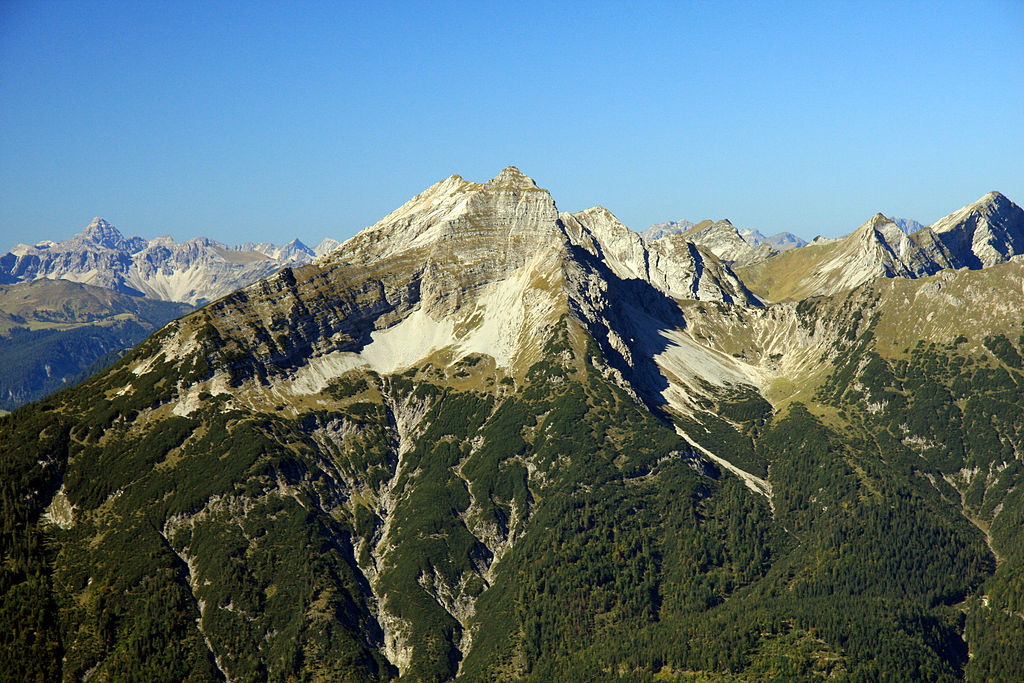
\includegraphics[width=0.5\textwidth]{pics/daniel.jpg} 
\caption{Szczyt Daniel}
\label{fig:Daniel}
\end{center}
\end{figure}

\begin{figure}[p]
\begin{center}
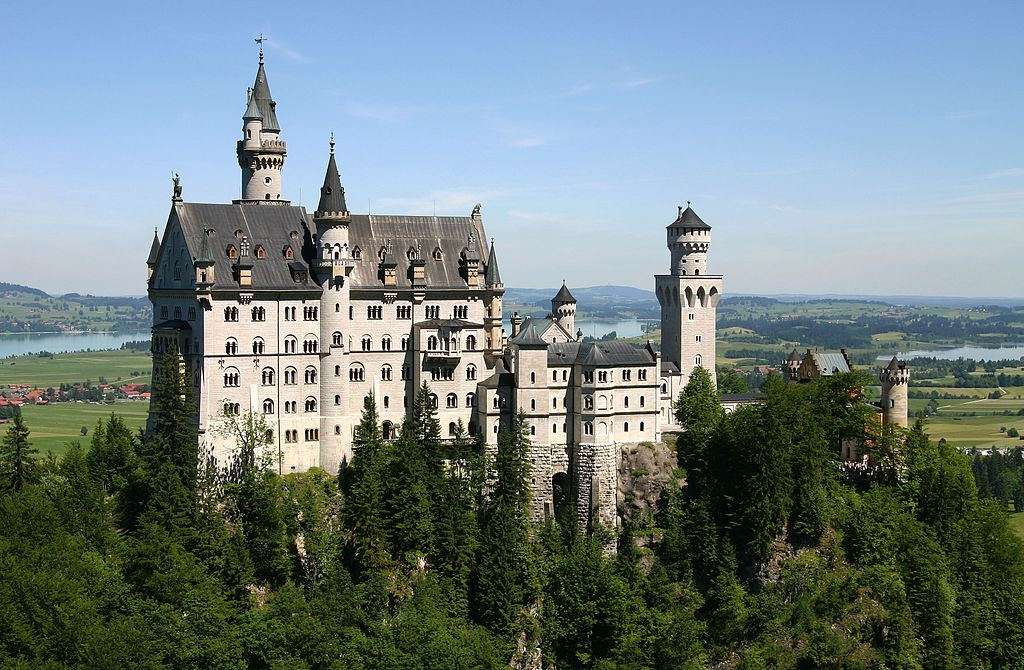
\includegraphics[width=0.5\textwidth]{pics/zamek.jpg} 
\caption{Zamek Neuschwanstein}
\label{fig:Zamek}
\end{center}
\end{figure}
\end{document}